\section{Testing the runtime}

\subsection{First stage testing}
A proper testing is needed for ensure the implementation work, before applying optimisation's and performance evaluation. I tested the runtime with the programs given, \texttt{tparallel.c}, \texttt{ttask.c} and \texttt{tsynchtasks.c}. Which where used during the development and when the final build is done, checking, it leads, to correct result.

\subsection{Testing with the mandelbrot set}
Also some algorithms where used for the testing. The first one was the mandelbrot set. I used the code given to check the output match. I modified the source code so it worked with the miniomp implementation (no single after parallel pragma needed) the version is called \texttt{tmandel-mini.c} and another version that works with the openmp implementation with name \texttt{tmandel-omp.c}. The following process was done to check the output matches:

\begin{figure}[h!]
    \centering
    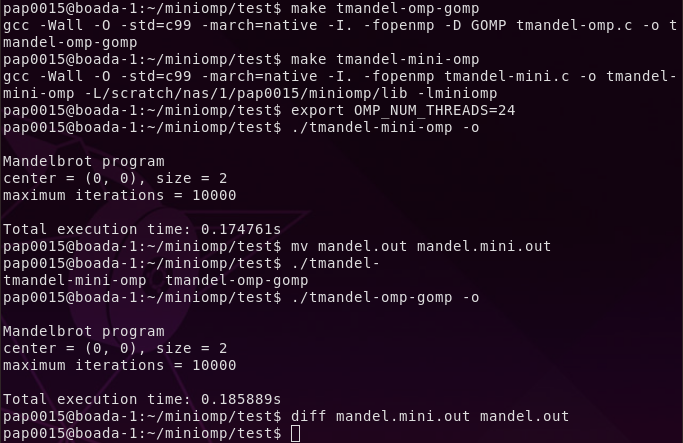
\includegraphics[width=0.9\textwidth]{mandelcheck.png}
    \caption{Check process for mandelbroot code}
\end{figure}

\subsection{Custom code for finding weak spots}
At this point we can tell that our implementation works well, but as a more strict testing is needed, I wrote a sample code to test all capabilities of the implementation and find some weak spots. 

\par ~\\
This program runs a set of tests to prove the synchronisation constructs which are the more likely to have bugs, also the other constructs are tested during the use of the synchronisation constructs.
\par ~\\
The program first of all initialises to vectors, one with $2^{10}$ elements the other with $2^9$ elements. Also we check the vectors are properly initialised with the \texttt{assert} function that checks sequentially that all values of the big vector match the argument, and with the \texttt{assert\_other} function we check the same but with the smaller vector.

\begin{lstlisting}[caption=Test initialisation code,label=testinit]
int main(int argc, char *argv[]) {
        int i, j;
        #pragma omp parallel 
        #ifdef GOMP
        #pragma omp single
        #endif
        {
                for( i = 0; i < (1 << 10); i++){
                        #pragma omp task firstprivate(i)
                        set(i, 1);
                }
                for( j = 0; j < (1 << 9); j++){
                        #pragma omp task firstprivate(j)
                        set_other(j, 1);
                }
                #pragma omp taskwait
                assert(1);
                assert_other(1);
\end{lstlisting}
\par ~\\
Then we perform a simple test, where we create $2^{10}$ tasks and then use taskwait to synchronise, also check that the value is the expected.

\begin{lstlisting}[caption=Simple taskwait test, label=testtaskwait]
                // TASKWAIT TEST
                for( i = 0; i < (1 << 10); i++){
                        #pragma omp task firstprivate(i)
                        compute_low(i);
                }
                #pragma omp taskwait
                assert(3900);
\end{lstlisting}
\par ~\\
Another simple test was running a taskgroup to wait to $2^{10}$ tasks. Checking the corresponding value at the end.
\begin{lstlisting}[caption=Simple taskgroup test, label=testtaskgroup]
                //TASKGROUP TEST
                #pragma omp taskgroup
                {
                for( i = 0; i < (1 << 10); i++){
                        #pragma omp task firstprivate(i)
                        compute_high(i); 
                }
                }
                assert(14649);
\end{lstlisting}
\par ~\\
A last test is performed. In order to check that taskgroup routine just waits for the tasks containing it and not the tasks created previously outside the taskgroup. With this purpose a first with a lot of computation work, then we create $2^9$ tasks inside a taskgroup, when the taskgroups ends, we check if the big task, has finished (leads to correct result) if not, then we can consider the test has succeded, because it means that the runtime when a taskgroup is encountered it just waits for the tasks created inside it. Then we check the taskgroup is properlly executed.
\begin{lstlisting}[caption=Taskgroup just waits for tasks created inside it test,label=testtaskgroupwait]
//BIG TASK AND THEN TASKGROUP TO CHECK RUNTIME DOESNT WAIT FOR OTHER TASKS
                #pragma omp task 
                for( i = 0; i < (1 << 10); i++){
                        add(i, -10000);
                        compute_high(i);
                        add(i, 10000);
                        compute_high(i);
                        add(i, -10000);
                }
                #pragma omp taskgroup
                for(j = 0; j < (1 << 9); j++){
                        #pragma omp task firstprivate(j)
                        compute_other(j);
                }
//THIS SHALL FAIL, PROOF OF TASKGROUP JUST WAITS FOR TASKGROUP TASKS
                assert(14649);
//THIS SHALL NOT FAIL
                assert_other(3900);
        }
}
\end{lstlisting}
\par ~\\
Executing the whole test code leads to expected output.
\begin{figure}[h!]
    \centering
    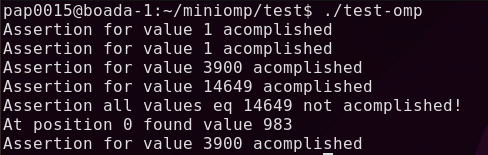
\includegraphics[width=0.7\textwidth]{testexec.png}
    \caption{Execution of the \texttt{test.c} code}
\end{figure}
\clearpage
\section{Performance evaluation}
\subsection{Tool for scalability analysis}
Before the performance evalution starts, I developed a tool that given to executables, one linked to miniomp and the other linked to openmp. The script can be found at \texttt{test/scalability.sh} folder in the root of the miniomp project. I will not be explaining the script as it is out of the scope of this document. 
\subsection{Performance evaluation with the mandelbrot set}
Using the tool seen in the last subsection, I executed a version linked to miniomp and a version linked to standard openmp.
\begin{figure}[h!]
    \centering
    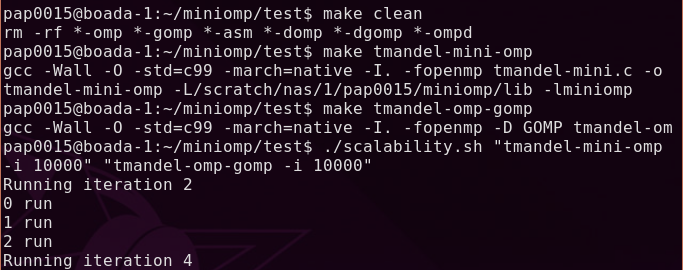
\includegraphics[width=0.7\textwidth]{scalabilitymandel.png}
    \caption{Execution of scalability script}
\end{figure}
\par ~\\
Obtaining the following results:
\begin{figure}[h!]
    \centering
    \includegraphics[width=0.9\textwidth]{output.png}
    \caption{Strong scalability plot for mandel}
\end{figure}
\par ~\\
We can see that both versions perform similar, but the miniomp runtime scales a bit better. Obviously, this is due to the restrictive miniomp implementation is, it doesn't have to track tasks generated by tasks to the taskgroup to work. Lets now get a trace to find more differences.

\par ~\\
Using extrae\footnote{Extrae: \url{tools.bsc.es/extrae}} to trace both programs running the mandel algorithm with 16 threads, and paraver\footnote{Paraver: \url{tools.bsc.es/paraver}} to visualize it. The general overview of both runs looks like this:

\begin{figure}[h!]
    \centering
    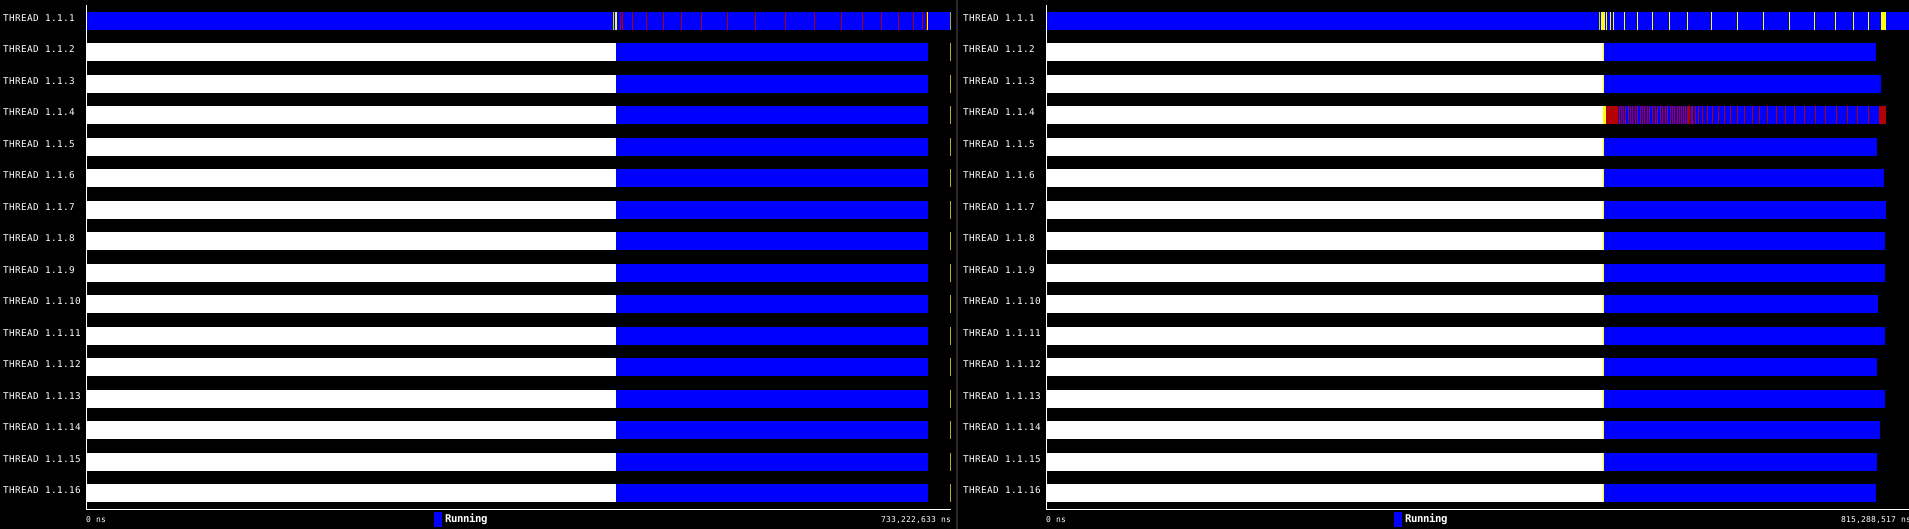
\includegraphics[width=1\textwidth]{paraver_general.png}
    \caption{General overview of both traced programs (left is miniomp, right is openmp}
\end{figure}
\par ~\\
Looking at the timescale, the first thing can be pointed out is that miniomp is a bit faster (as we seen in the scalability analysis). Also, miniomp, begins the parallel run (blue marks) at 0.45 seconds while the openmp begins at 0.5s. Another thing we can see is that, in the openmp run, the \texttt{thread 1.1.4} is chosen as the main thread, although, the \texttt{thread 1.1.1} is scheduling and fork/join. We can see this more clearly in \textit{hints->OpenMP->outlined function profiles} clicking on the histogram zoom, we get the following table that shows the time spend in parallel functions.

\par ~\\
As you can see, it can be clearly seen the implicit single inside the parallel construct implementation of miniomp, as just the first thread executes the parallel function. Also you can clearly see that in the openmp run, the \texttt{thread 1.1.4} is the main thread as it spends the most of the time in the parallel function. The last thing to comment out of this view is that miniomp runs the parallel region a bit faster, miniomp's main thread spends \texttt{0.264 seconds} and openmp main thread spends \texttt{0.266} seconds
\clearpage
\begin{figure}[htbp]
    \centering
    \includegraphics[width=0.4\textwidth]{paralleltime.png}
    \caption{Time in parallel, left miniomp, right openmp}
\end{figure}
\par ~\\
Now, we will take a look at the general view again. But zooming in, focusing on the initialisation of the parallel run, this includes, threads being created, initialised, and begin extracting tasks and executing. I zoomed in, to the part that the threads are created, in both runtimes, and fitted the time scale to the same.

\begin{figure}[htbp]
    \centering
    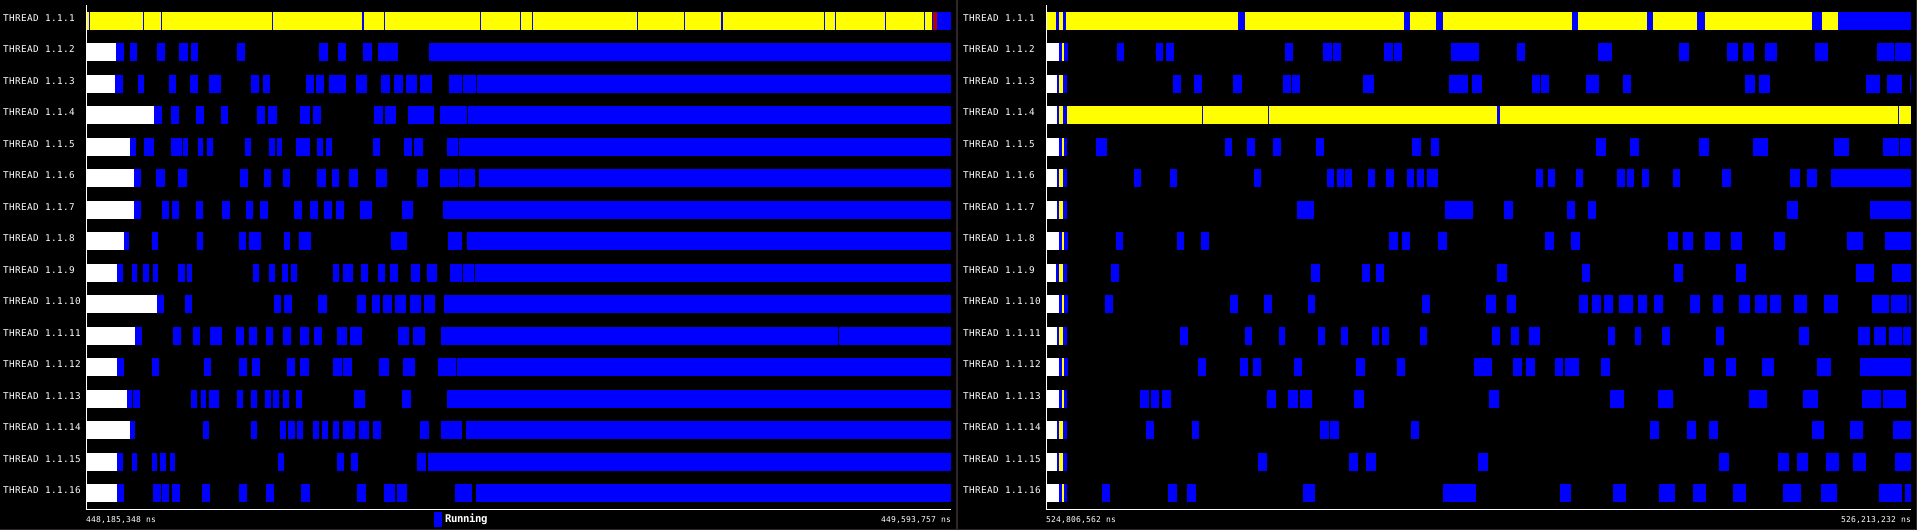
\includegraphics[width=1\textwidth]{init.png}
    \caption{Initialisation of the parallel region}
\end{figure}
\par ~\\
The main conclusion we can extract of this view is that miniomp is faster initialising the parallel region, there is less synchronization, less "black parts" (time not executing) and begins extracting and executing tasks much earlier. But we have to think of it, is the miniomp implementation more efficient? No, its not, what is happening is that miniomp, as mentioned before, is more restricted, and as it has lesser functionality such as the depend clauses, nested task synchronisation, it has to track much less information, much less data structures, and in consequence, it runs faster. 



